\documentclass[final,t]{beamer}
\mode<presentation>
{
%  \usetheme{Warsaw}
%  \usetheme{Aachen}
%  \usetheme{Oldi6}
%  \usetheme{I6td}
  \usetheme{I6dv}
%  \usetheme{I6pd}
%  \usetheme{I6pd2}
}
% additional settings
\setbeamerfont{itemize}{size=\normalsize}
\setbeamerfont{itemize/enumerate body}{size=\normalsize}
\setbeamerfont{itemize/enumerate subbody}{size=\normalsize}
% additional packages
\usepackage{ragged2e}
\usepackage{verbatim}
\usepackage{textcomp}
\usepackage[ampersand]{easylist}
\usepackage{lipsum}
\usepackage{times}
\usepackage{amsmath,amsthm, amssymb, latexsym}
\usepackage{exscale}
%\boldmath
\usepackage{booktabs, array}
%\usepackage{rotating} %sideways environment
\usepackage[english]{babel}
\usepackage[latin1]{inputenc}
\usepackage[orientation=landscape,size=custom,width=111.76,height=86.36,scale=1]{beamerposter}
\addtobeamertemplate{block begin}{}{\justifying}
\usepackage[export]{adjustbox}
\listfiles
\graphicspath{{figures/}}
% Display a grid to help align images
%\beamertemplategridbackground[1cm]

\title{\huge YAX: Taxonomic assignment using metagenomic shotgun sequences}
\author{Evan T. Bolyen$^{1}$, Mike R. DeBerg$^{1}$, Andrew J. Hodel$^{1}$, Hayden T. Westbrook$^{1}$, and Viacheslav Y. Fofanov$^{1}$}
\institute{$^{1}$School of Informatics, Computing, and Cyber Systems - Northern Arizona University}

% abbreviations
\usepackage{xspace}
\makeatletter
\DeclareRobustCommand\onedot{\futurelet\@let@token\@onedot}
\def\@onedot{\ifx\@let@token.\else.\null\fi\xspace}
\def\eg{{e.g}\onedot} \def\Eg{{E.g}\onedot}
\def\ie{{i.e}\onedot} \def\Ie{{I.e}\onedot}
\def\cf{{c.f}\onedot} \def\Cf{{C.f}\onedot}
\def\etc{{etc}\onedot}
\def\vs{{vs}\onedot}
\def\wrt{w.r.t\onedot}
\def\dof{d.o.f\onedot}
\def\etal{{et al}\onedot}
\makeatother

%%%%%%%%%%%%%%%%%%%%%%%%%%%%%%%%%%%%%%%%%%%%%%%%%%%%%%%%%%%%%%%%%%%%%%%%%%%%%%%%%%%%%%%%%%%%%%%%%%%%%%%%%%%%
%%%%%%%%%%%%%%%%%%%%%%%%%%%%%%%%%%%%%%%%%%%%%%%%%%%%%%%%%%%%%%%%%%%%%%%%%%%%%%%%%%%%%%%%%%%%%%%%%%%%%%%%%%%%
\begin{document}
\begin{frame}{}
  \begin{columns}[t]
    \begin{column}{.3\linewidth}
        \begin{alertblock}{
\includegraphics[width=.8\linewidth]{assets/yak}\newline\newline}
            YAX is a both a tool for taxonomic classification and a computational pipeline manager.\newline
        \end{alertblock}
        \begin{block}{Problem Statement}
            Traditional taxonomic assignment techniques are time consuming (sometimes taking weeks)
            making transient failures likely, additionally there are many possible parameters to adjust.
        \end{block}
        \begin{block}{Requirements}
            \textbf{Modular}
            \begin{itemize}
                \item[$\bullet$]Incorporate developing technologies
                \item[$\bullet$]Evaluate different processes
            \end{itemize}
            \vspace{0.5cm}
            \textbf{Fail Early}
            \begin{itemize}
                \item[$\bullet$]Validate parameters and dependencies before running
                \item[$\bullet$]Prevent failure in the middle of a run for spurious reasons
            \end{itemize}
            \vspace{0.5cm}
            \textbf{Coverage Representation}
            \begin{itemize}
                \item[$\bullet$]Provide biologists with relevant details
                \item[$\bullet$]Every identified taxon is qualified with coverage data
            \end{itemize}
            \vspace{0.5cm}
            \textbf{State System}
            \begin{itemize}
                \item[$\bullet$]Manage component requirements
                \item[$\bullet$]Control and record all data produced
                \item[$\bullet$]Eliminates redundant recomputation
                \item[$\bullet$]Allows parameter exploration
            \end{itemize}
        \end{block}

        \begin{block}{Managing State}
            The figure below represents multiple runs of a pipeline. By using a state-system, YAX is able to identify where parameters are shared and reuse the results. \\
            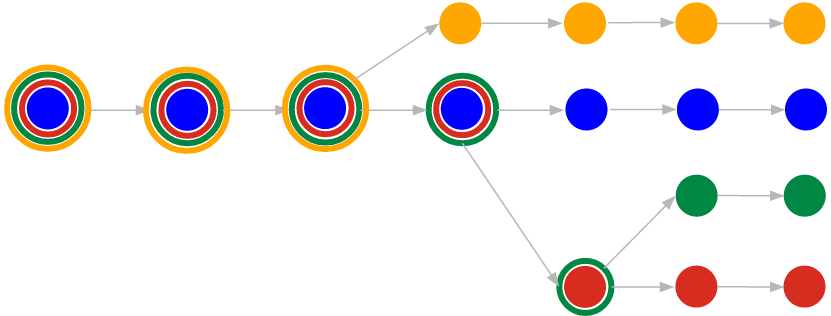
\includegraphics[width=1\linewidth]{assets/Artifacts}
        \end{block}

      %%%%%%%%%%%%%%%%%%%%%%%%%%%%%%%%%%%%%%%%%%%%%%%%%%%%%%%%%%%%%%%%%%%%%%%%%%%%%%%%%%%%%%%%%%%%%%%%%%%%%%%%%%%%


    \end{column}
    \begin{column}{.3\linewidth}
        %%%%%%%%%%%%%%%%%%%%%%%%%%%%%%%%%%%%%%%%%%%%%%%%%%%%%%%%%%%%%%%%%%%%%%%%%%%%%%%%%%%%%%%%%%%%%%%%%%%%%%%%%%%%


        \begin{block}{Assigning Taxonomy}
            \textbf{Use strict matching against the entire reference set to remove obviously wrong results:}\\
            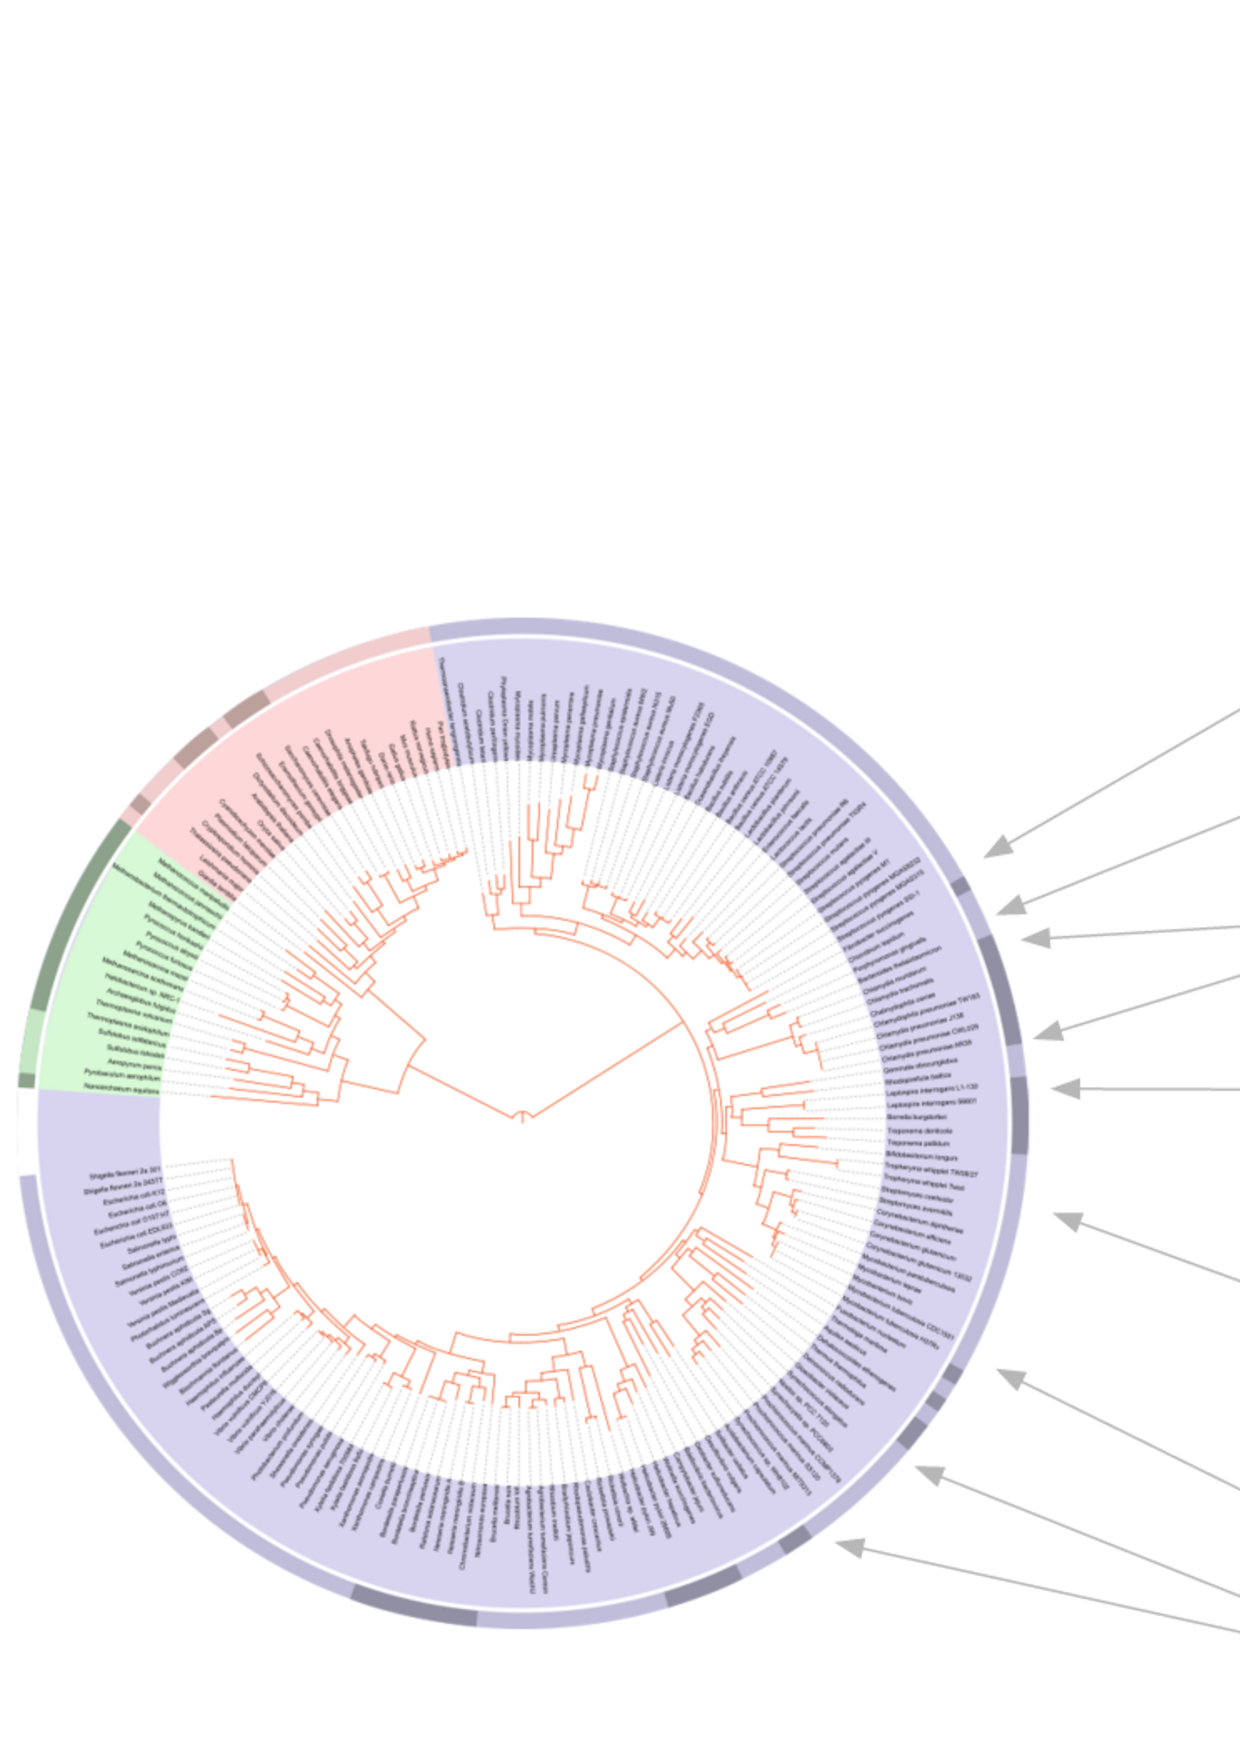
\includegraphics[width=.8\linewidth, right]{assets/Whole} \\
            \textbf{Using the results from the last step, perform a detailed\\ refinement with looser parameters:}
            \begin{columns}
                \begin{column}{.42\linewidth}
                    \begin{minipage}{\linewidth}
                        \begin{itemize}
                            \huge
                            \item[$\bullet$]\huge\textbf{1.6 Terabases}
                            \item[$\bullet$]\huge\textbf{200 Gigabases}
                            \item[$\bullet$]\huge\textbf{1.6 Sextillion Comparisons}
                        \end{itemize}
                    \end{minipage}
                \end{column}
                \begin{column}{.55\linewidth}
                    \begin{minipage}{\linewidth}
                        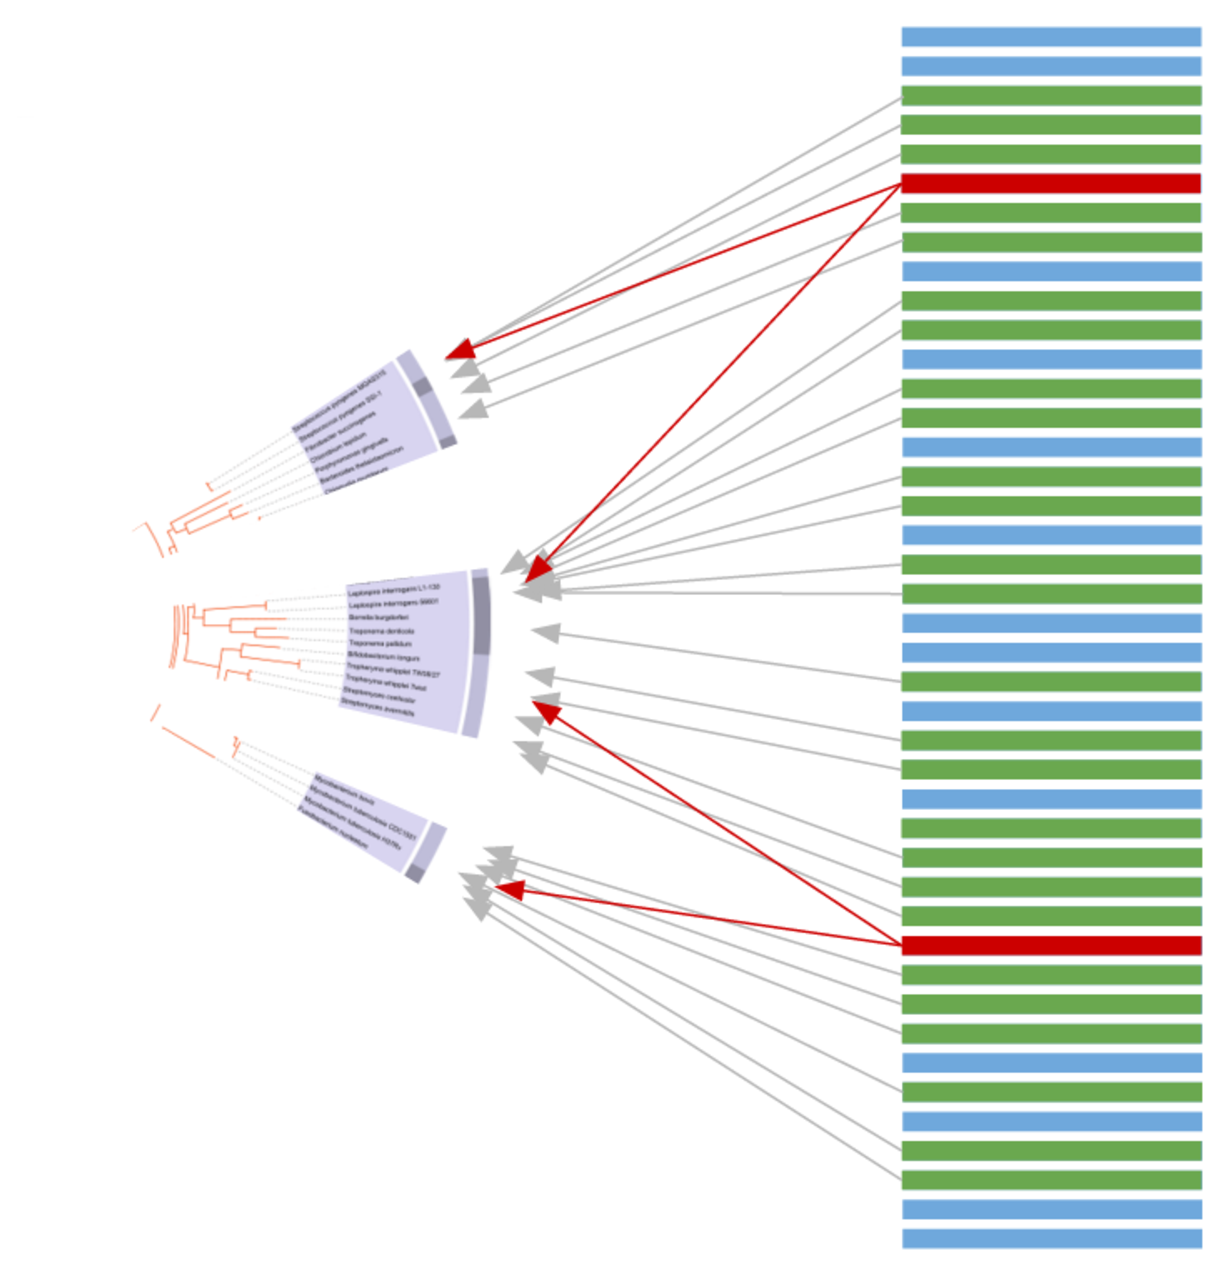
\includegraphics[width=.99\linewidth, right]{assets/Subset}
                    \end{minipage}
                \end{column}
            \end{columns}
        \end{block}
        \begin{block}{Making Sense of the Results}
            In order to leverage the expertise of trained biologists, we provide plots which represent the coverage
            of a target genome by reads from the sample set.\newline\newline
        \textbf{Good Coverage:}\\
        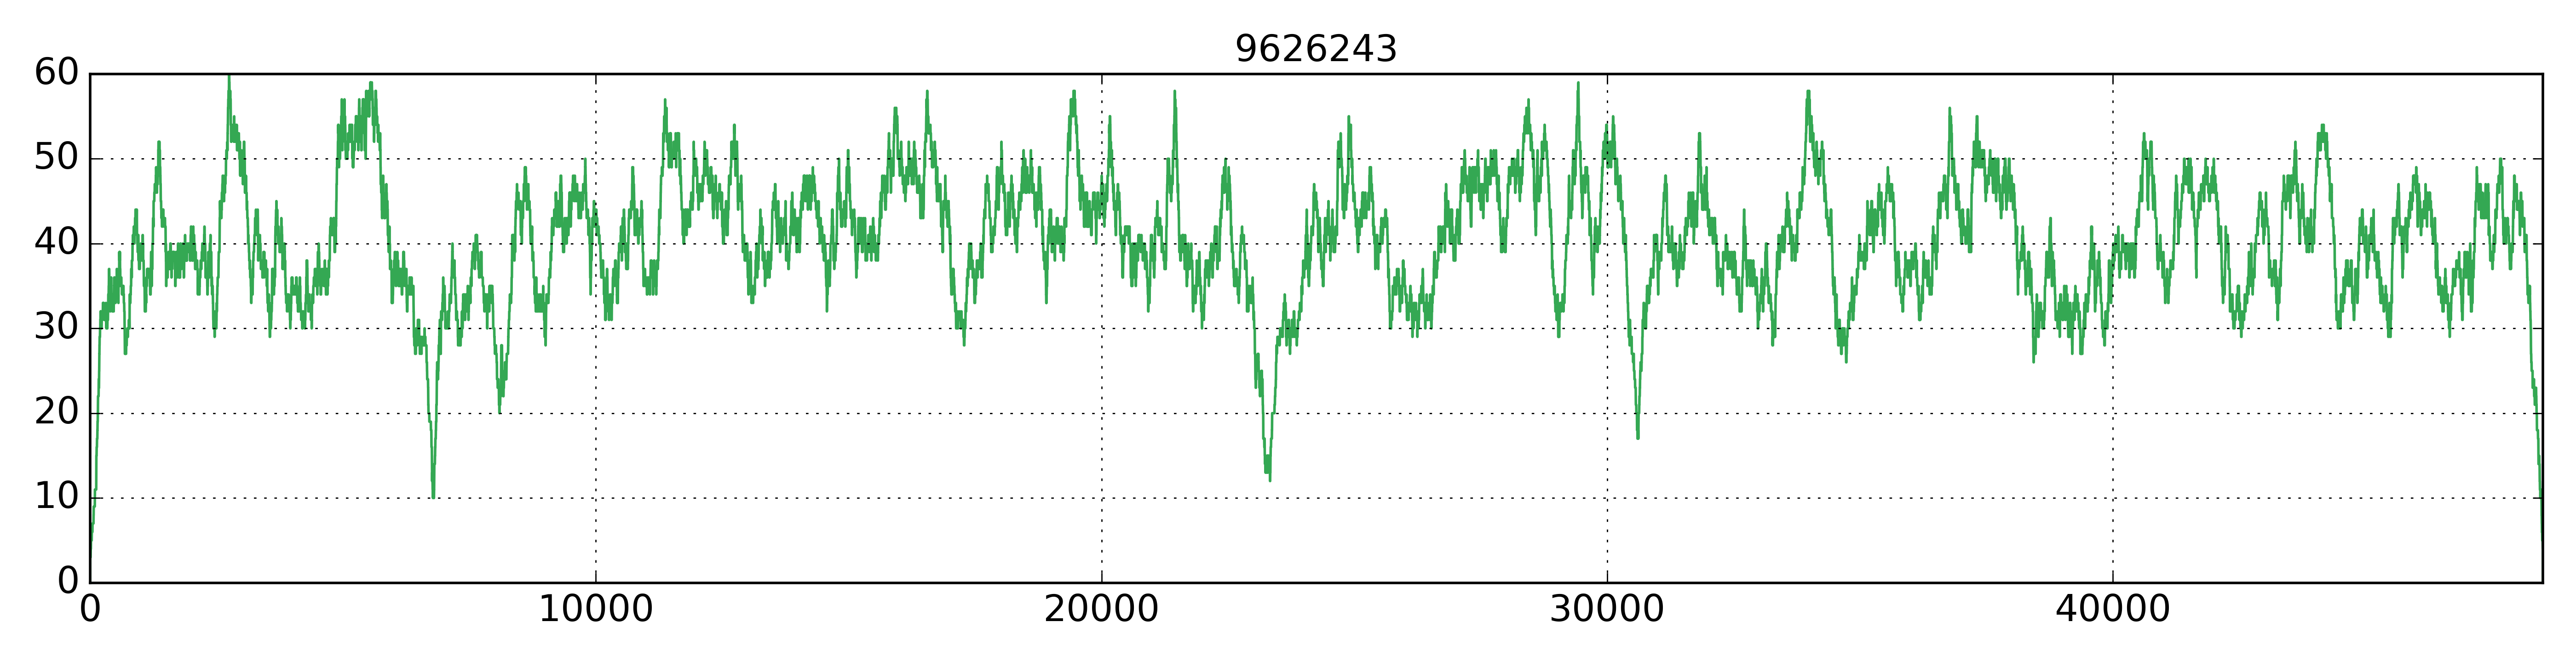
\includegraphics[width=.95\linewidth, center]{assets/coverage_plot_good}\\
        \textbf{Bad Coverage:}\\
        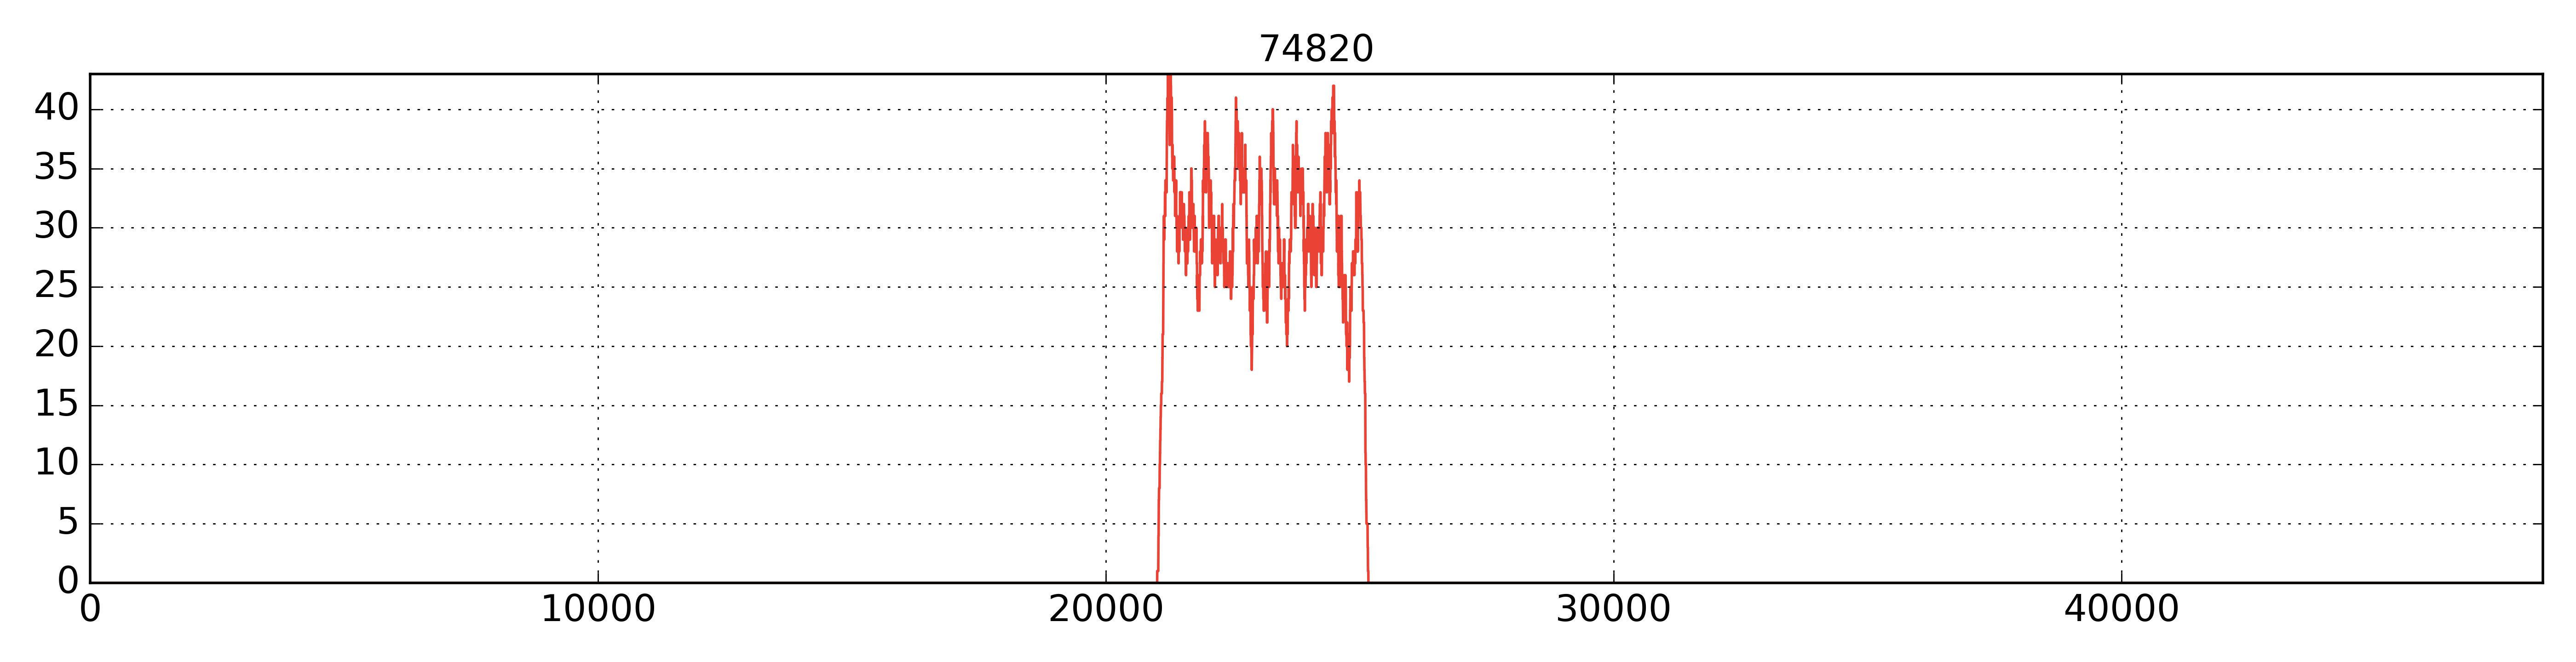
\includegraphics[width=.95\linewidth, center]{assets/coverage_plot_bad}
        \end{block}

    \end{column}

    %%%%%%%%%%%%%%%%%%%%%%%%%%%%%%%

    \begin{column}{.3\linewidth}
        \begin{block}{Architecture}
            A YAX architectural configuration file is used to initialize the topology of a pipeline, build the
            ExeGraph, and a database which will store Artifacts (an intermediate result).
            The ExeGraph represents the behavior of the pipeline, interacting with functional Modules via ExeNodes preventint
            coupling by disassociating Modules from each other and the pipeline. The database is managed by IndianaJones
            (named after the dog) who is responsible for managing the existing
            Artifacts so that they may be reused in subsequent runs of this pipeline. \newline
            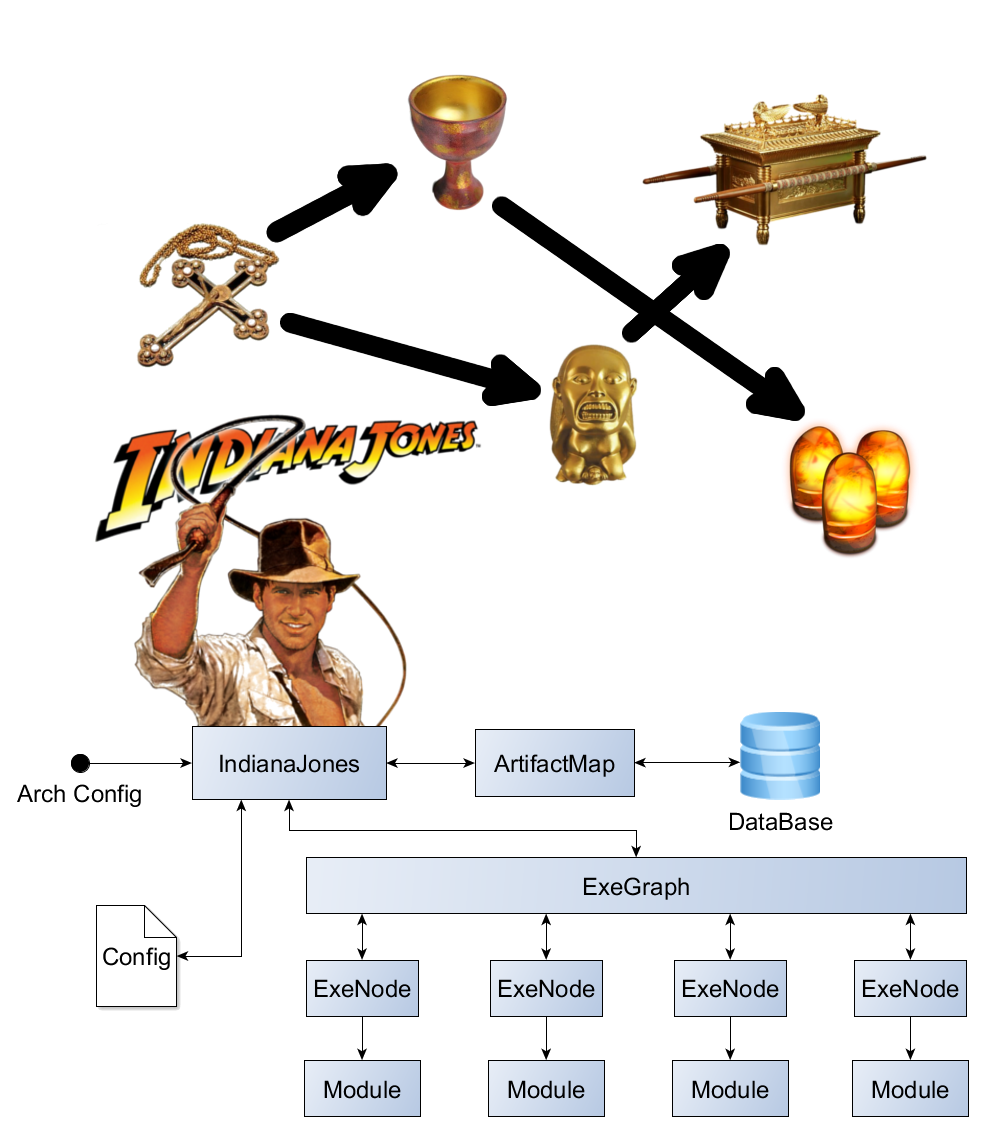
\includegraphics[width=.95\linewidth]{assets/arch}
        \end{block}

        \begin{block}{Future Work}
            YAX is designed to be highly modular, capable of adapting with technological development. As part of its development
            YAX was built to not only provide one solution, but to allow exploration between different possible solutions.

        \end{block}
        \begin{block}{Facilitating Technologies}
        \begin{itemize}
            \small
            \item[$\bullet$]Python 3.5 - An excellent language, much better than Python 2.7
            \item[$\bullet$]Bowtie2 - Fast and accurate alignment
            \item[$\bullet$]Bowtie2-mg - Bowtie2 wrapper for metagenomic binning
            \item[$\bullet$]ReadPrep - Raw sequence FASTQ file processing
            \item[$\bullet$]TaxIDTool - Manages taxonomic trees
            \item[$\bullet$]Matplotlib - Plotting library
            \item[$\bullet$]PDFKit - Creating rendered output
            \item[$\bullet$]Miniconda - Packaging and environment management
            \item[$\bullet$]TravisCI - Continuous integration service
            \item[$\bullet$]git and GitHub - Version control software and hosting
        \end{itemize}
        \end{block}

        %%%%%%%%%%%%%%%%%%%%%%%%%%%%%%%%%%%%%%%%%%%%%%%%%%%%%%%%%%%%%%%%%%%%%%%%%%%%%%%%%%%%%%%%%%%%%%%%%%%%%%%%%%%%



%%%%%%%%%%%%%%%%%%%%%%%%%%%%%%%%%%%%%%%%%%%%%%%%%%%%%%%

    \end{column}
  \end{columns}

\end{frame}

\end{document}


%%%%%%%%%%%%%%%%%%%%%%%%%%%%%%%%%%%%%%%%%%%%%%%%%%%%%%%%%%%%%%%%%%%%%%%%%%%%%%%%%%%%%%%%%%%%%%%%%%%%
%%% Local Variables:
%%% mode: latex
%%% TeX-PDF-mode: t
%%% End:
